% Artigo do TP de Banco de Dados II — template JAES (jaes.cls)
\documentclass{jaes}

% Metadata
\jyear{2026}
\jmonth{July}

\usepackage[brazil]{babel}
\usepackage{microtype}
\usepackage{listings}
\usepackage{tikz}
\usetikzlibrary{positioning,arrows.meta,fit,shapes.multipart,shapes.geometric,calc,babel}

\sloppy

% ---- cabeçalho/rodapé: troca os marcadores DRAFT pela data de compilação ----
\makeatletter
\def\ps@headings{%
    \def\@evenhead{{\rhfont\leftmark}\hfil}%
    \def\@oddhead{\hfil{\rhfont\rightmark}}%
    \def\@evenfoot{\hbox to \textwidth{\rhfont\evenfolio\hfill}}%
    \def\@oddfoot{\hbox to \textwidth{\rhfont\hfill\oddfolio}}%
    \let\@mkboth\markboth
    \def\chaptermark##1{\markboth{##1}{##1}}}
\def\ps@plain{\let\@mkboth\@gobbletwo
    \def\@evenhead{}%
    \def\@oddhead{}%
    \def\@evenfoot{\hbox to \textwidth{\rhfont\thepage\hfill}}%
    \def\@oddfoot{\hbox to \textwidth{\rhfont\hfill\thepage}}}
% remove a seção "THE AUTHORS" (biografias) do final do artigo
\def\printbiography{}
\makeatother
\pagestyle{headings}

% permite empilhar duas figuras largas no topo da mesma página
\renewcommand{\dbltopfraction}{0.95}
\renewcommand{\dblfloatpagefraction}{0.6}
\setcounter{dbltopnumber}{3}

% ---- estilos TikZ das figuras ----
\tikzset{
  comp/.style={draw, rounded corners=2pt, fill=black!4, font=\small\sffamily,
    align=center, minimum height=8mm, inner sep=5pt},
  store/.style={draw, cylinder, shape border rotate=90, aspect=0.12,
    fill=black!8, font=\small\sffamily, align=center, inner sep=5pt},
  ext/.style={comp, fill=white, densely dashed},
  layer/.style={comp, minimum width=27mm},
  group/.style={draw, rounded corners=3pt, inner sep=7pt, densely dotted},
  grouplabel/.style={font=\footnotesize\sffamily\bfseries, anchor=south west},
  flow/.style={-{Stealth[length=2.4mm]}, semithick},
  flowlabel/.style={font=\scriptsize\sffamily, fill=white, inner sep=1.5pt, midway},
  class/.style={draw, rectangle split, rectangle split parts=2,
    rectangle split part fill={black!12, white}, font=\scriptsize\sffamily,
    inner sep=3.4pt, execute at begin node=\renewcommand{\arraystretch}{0.92}},
  rel/.style={-{Stealth[length=2.2mm]}, semithick},
  rellabel/.style={font=\tiny\sffamily\bfseries, fill=white, inner sep=1.2pt, midway},
  life/.style={draw, fill=black!8, font=\small\sffamily, minimum height=7mm,
    minimum width=23mm},
  msg/.style={-{Stealth[length=2.2mm]}, semithick},
  msglabel/.style={font=\scriptsize\sffamily, midway, above=0.3mm},
  retmsg/.style={-{Stealth[length=2.2mm]}, semithick, densely dashed},
}

% ---- listagens Cypher ----
\lstdefinelanguage{Cypher}{
  morekeywords={MATCH,OPTIONAL,WHERE,RETURN,CREATE,MERGE,SET,DELETE,DETACH,
    WITH,UNWIND,ORDER,BY,SKIP,LIMIT,AS,AND,OR,NOT,IN,ON,CONSTRAINT,REQUIRE,
    UNIQUE,FOR,IS,EXISTS},
  sensitive=true,
  morecomment=[l]{//},
  morestring=[b]',
}
\lstset{
  language=Cypher,
  basicstyle=\small\ttfamily,
  keywordstyle=\bfseries\color{blue!55!black},
  stringstyle=\color{red!65!black},
  commentstyle=\itshape\color{black!55},
  columns=fullflexible,
  keepspaces=true,
  frame=single,
  rulecolor=\color{black!35},
  breaklines=true,
  captionpos=b,
  abovecaptionskip=4pt,
  belowcaptionskip=14pt,
  aboveskip=10pt,
  belowskip=8pt,
}
\renewcommand{\lstlistingname}{Query}

% cores dos tipos de dados na Fig. do modelo
\colorlet{tString}{red!75!black}
\colorlet{tInt}{blue!75!black}
\colorlet{tFloat}{teal!70!black}
\colorlet{tUUID}{violet!85!black}
\colorlet{tPoint}{orange!80!black}
\colorlet{tBool}{brown!80!black}
\newcommand{\tstr}{\textcolor{tString}{String}}
\newcommand{\tint}{\textcolor{tInt}{Integer}}
\newcommand{\tflt}{\textcolor{tFloat}{Float}}
\newcommand{\tuid}{\textcolor{tUUID}{UUID}}
\newcommand{\tpnt}{\textcolor{tPoint}{Point}}
\newcommand{\tbol}{\textcolor{tBool}{Boolean}}

\begin{document}

% Title portion
\title{Cachaceiro Viajante: Um Sistema Baseado em Grafos para o Planejamento de Rotas entre Alambiques de Minas Gerais}

% Page heads {Authors}{Short title}
\markboth{CAMILO ET AL.}{CACHACEIRO VIAJANTE}

% Author Info.
\authorgroup{
\author{EDUARDA GOMES CAMILO,\textsuperscript{1}}
AND \author{GUILHERME FERREIRA,\textsuperscript{1}}
AND \author{GUILHERME OLIVEIRA\textsuperscript{1}}
\email{(\{eduarda.camilo, guilherme.ff, guilherme.os1\}@aluno.ufop.edu.br)}
\affil{\textsuperscript{1}Instituto de Ciências Exatas e Aplicadas, Universidade Federal de Ouro Preto (UFOP), João Monlevade, MG, Brasil}
}

% Abstract
\abstract{%
Este artigo apresenta o desenvolvimento do Cachaceiro Viajante, uma aplicação para consulta de alambiques e planejamento de roteiros de visita em Minas Gerais, construída como resposta ao problema de organizar informações fortemente conectadas do domínio turístico e gerar percursos entre estabelecimentos. A solução utiliza o banco de dados não relacional Neo4j para representar usuários, avaliações, alambiques e cidades por meio de nós e relacionamentos. O sistema permite consultar estabelecimentos, registrar avaliações, indicar novos alambiques e gerar uma ordem aproximada de visita usando as heurísticas de vizinho mais próximo e 2-opt, enquanto o OSRM fornece a geometria viária exibida em um mapa interativo. A aplicação também agrupa os alambiques em circuitos naturais de visita por meio do algoritmo evolutivo multiobjetivo de detecção de comunidades HP-MOCD, disponibilizado pela biblioteca pymocd, executado sobre um grafo de proximidade derivado das coordenadas armazenadas. O trabalho demonstra uma aplicação prática de bancos de dados em grafos e de análise de redes em um domínio turístico.}
\maketitle

\section{Introdução}

O planejamento de uma visita a diferentes pontos de interesse envolve a organização de informações como localização, distância, características dos estabelecimentos e ordem de deslocamento. Determinar a ordem de visita que minimiza o deslocamento total é um problema clássico de otimização combinatória, conhecido como Problema do Caixeiro Viajante (TSP) \cite{applegate2006tsp}. Assim, quando vários destinos são considerados, a definição manual de um roteiro pode se tornar uma tarefa complexa, principalmente quando as informações estão distribuídas e não se dispõe de uma ferramenta que concentre a consulta dos locais e a geração do percurso.

No contexto do turismo relacionado aos alambiques de Minas Gerais, os dados possuem uma natureza fortemente conectada. Alambiques estão associados a cidades, recebem avaliações de usuários e podem ser incluídos na plataforma por meio de indicações. Sistemas de bancos de dados em grafos, como o Neo4j, são adequados a aplicações que demandam o percurso frequente das referências existentes entre elementos relacionados \cite{cattell2010scalable}.

Diante desse contexto, este trabalho busca responder à seguinte questão: como um banco de dados em grafos pode ser utilizado para organizar informações sobre alambiques e apoiar o planejamento de uma rota de visita entre diferentes estabelecimentos? O objetivo geral consiste em desenvolver uma aplicação que permita consultar alambiques, registrar avaliações, indicar novos estabelecimentos, gerar uma ordem de visita entre destinos selecionados pelo usuário e sugerir circuitos de visita obtidos automaticamente por detecção de comunidades sobre o grafo de proximidade dos estabelecimentos \cite{Santos2025}.

Para atender a esse objetivo, foi desenvolvido o Cachaceiro Viajante, uma aplicação que utiliza o Neo4j para armazenar os dados relacionados a usuários, alambiques, cidades e avaliações. A solução possui uma interface para consulta e seleção dos estabelecimentos, um backend responsável pelas regras de negócio e pelo acesso ao banco de dados e um mecanismo de planejamento que aplica heurísticas para determinar uma ordem aproximada de visita.

O desenvolvimento do sistema compreendeu o levantamento das funcionalidades, a elaboração dos modelos conceitual e lógico, a implementação do banco de dados em grafos, a construção da interface e do backend e a integração dos componentes da aplicação. O acesso ao Neo4j foi realizado por meio de seu driver oficial e de consultas escritas na linguagem Cypher.

O restante deste artigo está organizado da seguinte forma. A Seção~2 apresenta a arquitetura, a escolha do Neo4j, a modelagem dos dados, a lógica de planejamento das rotas e a detecção de comunidades utilizada na sugestão de circuitos. A Seção~3 descreve a implementação do backend, do frontend, do serviço de detecção de comunidades e o ambiente utilizado no desenvolvimento. Por fim, a Seção~4 apresenta as considerações finais e as possibilidades de evolução do sistema.

\section{Arquitetura e Modelagem do Sistema}

A aplicação é composta por um frontend web, um backend organizado em camadas, um microsserviço de detecção de comunidades e o banco de dados Neo4j, além do serviço externo OSRM para a geometria viária. A Fig.~\ref{fig:arquitetura} apresenta a visão geral dos componentes e das comunicações entre eles.

\begin{figure*}[t]
\centering
\begin{tikzpicture}[node distance=9mm and 12mm]
  % frontend
  \node[comp, minimum width=34mm] (ui) {Telas e componentes\\{\scriptsize (catálogo, rotas, avaliações, mapa Leaflet)}};
  \node[group, fit=(ui)] (fe) {};
  \node[grouplabel] at (fe.north west) {Frontend};
  % backend layers
  \node[layer, right=22mm of ui, yshift=16mm] (rt) {Routes\\{\scriptsize /auth\ \ /distilleries\ \ /reviews}\\{\scriptsize /routes\ \ /stats\ \ /communities}};
  \node[layer, below=4mm of rt] (ct) {Controllers};
  \node[layer, below=4mm of ct] (sv) {Services\\{\scriptsize regras de negócio, TSP,}\\{\scriptsize circuitos (kNN)}};
  \node[layer, below=4mm of sv] (md) {Models\\{\scriptsize consultas Cypher}};
  \node[group, fit=(rt)(ct)(sv)(md)] (be) {};
  \node[grouplabel] at (be.north west) {Backend};
  % stores and services
  \node[store, right=20mm of md, minimum width=26mm] (db) {Neo4j~5\\{\scriptsize grafo de propriedades}\\{\scriptsize e pontos espaciais}};
  \node[comp, right=20mm of sv, minimum width=26mm, yshift=10mm] (comm) {app-community\\{\scriptsize Python / Flask}\\{\scriptsize HP-MOCD (pymocd)}};
  \node[ext, below=10mm of ui, minimum width=30mm] (osrm) {OSRM\\{\scriptsize roteamento OpenStreetMap}};
  % flows
  \draw[flow] (ui.east) -- node[flowlabel]{HTTP/JSON} (rt.west);
  \draw[flow] (rt) -- (ct);
  \draw[flow] (ct) -- (sv);
  \draw[flow] (sv) -- (md);
  \draw[flow] (md.east) -- node[flowlabel]{Bolt / Cypher} (db.west);
  \draw[flow] (sv.east) -- node[flowlabel]{arestas kNN} (comm.west);
  \draw[flow] (ui.south) -- node[flowlabel]{geometria viária} (osrm.north);
\end{tikzpicture}
\caption{Arquitetura do sistema Cachaceiro Viajante: o frontend consome a API do backend, que acessa o Neo4j via Cypher e delega a detecção de comunidades ao microsserviço Python; o OSRM fornece a geometria das estradas diretamente ao frontend.}
\label{fig:arquitetura}
\end{figure*}

\subsection{Escolha do Neo4j}

A escolha do sistema gerenciador de banco de dados foi realizada considerando a estrutura do domínio do Cachaceiro Viajante. A aplicação reúne usuários, avaliações, alambiques e cidades, cujas associações possuem papel central nas funcionalidades oferecidas. Um usuário pode escrever diferentes avaliações, uma avaliação está associada a um alambique, os alambiques estão localizados em cidades e novos estabelecimentos podem ser indicados pelos usuários.

No modelo orientado a grafos, os dados são representados por meio de nós, relacionamentos e propriedades, permitindo que as associações sejam tratadas de forma nativa \cite{monteiro2026grafos}. Essa estrutura favorece aplicações que realizam navegação frequente entre elementos relacionados \cite{cattell2010scalable}.

Diante dessas características, foi adotado o Neo4j. Além da representação dos relacionamentos, o SGBD disponibiliza o tipo espacial \texttt{point}, utilizado no projeto para armazenar as coordenadas geográficas dos alambiques e das cidades. As operações de persistência são realizadas diretamente na linguagem Cypher, por meio do driver oficial do Neo4j.

\subsubsection{Por que não utilizar uma abordagem relacional?}

Uma implementação baseada em banco de dados relacional seria tecnicamente possível. Nesse caso, usuários, avaliações, alambiques e cidades seriam representados por tabelas, enquanto as associações entre esses elementos dependeriam de chaves estrangeiras e, em alguns casos, de tabelas intermediárias.

Entretanto, como as relações entre os elementos possuem importância central no domínio da aplicação, sua representação em um grafo torna-se mais direta. No Neo4j, relacionamentos como \texttt{WROTE}, \texttt{ABOUT}, \texttt{LOCATED\_IN}, \texttt{SUGGESTED} e \texttt{ROAD} fazem parte da própria estrutura armazenada, podendo possuir direção e propriedades.

A escolha do modelo em grafos não decorre de uma impossibilidade de uso do modelo relacional, mas de sua maior aderência à estrutura conectada dos dados do Cachaceiro Viajante. Dessa forma, é possível representar explicitamente as associações do domínio e realizar consultas que percorrem esses relacionamentos por meio da linguagem Cypher.

\subsubsection{Modelo Conceitual e Lógico}

\textbf{Modelo conceitual.}
No nível conceitual, o modelo foi estruturado a partir de quatro elementos principais: usuário, alambique, cidade e avaliação. As relações entre esses elementos representam a autoria das avaliações, os estabelecimentos avaliados, a localização dos alambiques, as indicações realizadas pelos usuários e as conexões existentes entre as cidades. A Fig.~\ref{fig:modelo-logico} apresenta o diagrama do modelo de dados, em notação baseada no diagrama de classes UML, reunindo as entidades, suas propriedades e os relacionamentos do domínio.

\begin{figure*}[t]
\centering
\begin{tikzpicture}[node distance=8mm and 12mm]
  \node[class] (user) {\textbf{User}
    \nodepart{two}\begin{tabular}{@{}l@{}}
      id: \tuid\\ name: \tstr\\ username: \tstr\\ email: \tstr\\
      passwordHash: \tstr\\ reputation: \tflt\\ createdAt: \tstr\\ updatedAt: \tstr
    \end{tabular}};
  \node[class, right=12mm of user.north east, anchor=north west] (review) {\textbf{Review}
    \nodepart{two}\begin{tabular}{@{}l@{}}
      id: \tuid\\ title: \tstr\\ body: \tstr\\ rating: \tflt\\ createdAt: \tstr
    \end{tabular}};
  \node[class, right=12mm of review.north east, anchor=north west] (dist) {\textbf{Distillery}
    \nodepart{two}\begin{tabular}{@{}l@{}}
      id: \tuid\\ name: \tstr\\ category: \tstr\\ status: \tstr\\ rating: \tflt\\
      reviewCount: \tint\\ founded: \tint\\ signature: \tstr\\ tags: \tstr[]\\
      landmark: \tbol\\ location: \tpnt\\ createdAt: \tstr\\ updatedAt: \tstr
    \end{tabular}};
  \node[class, right=12mm of dist.north east, anchor=north west] (city) {\textbf{City}
    \nodepart{two}\begin{tabular}{@{}l@{}}
      name: \tstr\\ region: \tstr\\ location: \tpnt
    \end{tabular}};
  \draw[rel] (user.east |- review.150) -- node[rellabel]{WROTE} node[below=1.5mm, font=\tiny\sffamily, midway]{1 $\rightarrow$ 0..*} (review.150);
  \draw[rel] (review.east |- review.150) -- node[rellabel]{ABOUT} node[below=1.5mm, font=\tiny\sffamily, midway]{0..* $\rightarrow$ 1} (dist.west |- review.150);
  \draw[rel] (dist.east |- city.150) -- node[rellabel]{LOCATED\_IN} node[below=1.5mm, font=\tiny\sffamily, midway]{0..* $\rightarrow$ 1} (city.150);
  \draw[rel] (user.south) |- node[rellabel, pos=0.75]{SUGGESTED}
    node[below=1.5mm, font=\tiny\sffamily, pos=0.75]{0..* $\rightarrow$ 0..*}
    ($(dist.south)+(0,-7mm)$) -- (dist.south);
  \draw[rel] ($(city.north)+(3mm,0)$) -- ++(0,4mm)
    -| node[rellabel, pos=0.25, above=0.6mm]{ROAD (km)\ \ 0..* $\rightarrow$ 0..*}
    ($(city.east)+(7mm,0)$) -- (city.east);
\end{tikzpicture}
\caption{Modelo de dados do banco orientado a grafos: nós \textsf{User}, \textsf{Review}, \textsf{Distillery} e \textsf{City} com seus principais atributos e os relacionamentos do domínio.}
\label{fig:modelo-logico}
\end{figure*}

\textbf{Modelo lógico.}
No modelo lógico em grafos, esses elementos foram implementados pelos nós \texttt{User}, \texttt{Distillery}, \texttt{City} e \texttt{Review}. Os relacionamentos \texttt{WROTE} e \texttt{ABOUT} conectam o autor, a avaliação e o estabelecimento avaliado. O relacionamento \texttt{LOCATED\_IN} associa um alambique à sua cidade, enquanto \texttt{SUGGESTED} registra a indicação de um estabelecimento por um usuário. O relacionamento \texttt{ROAD} representa conexões entre cidades e pode armazenar a distância estimada entre elas.

Foram definidas restrições de unicidade para o e-mail e o nome de usuário dos usuários, para o identificador e o nome dos alambiques, para o nome das cidades e para o identificador das avaliações.

\subsection{Backend}

O backend foi organizado em rotas, controladores, serviços e modelos. As rotas definem os endpoints disponíveis e encaminham as requisições recebidas. Os controladores extraem os dados das requisições, acionam os serviços correspondentes e preparam as respostas HTTP.

Os serviços concentram a validação dos dados e as regras de negócio, como o cadastro de usuários, o registro de avaliações, a indicação de alambiques e o planejamento das rotas. Nessa camada também são executadas as heurísticas utilizadas para determinar a ordem aproximada de visita.

Os modelos são responsáveis pela comunicação com o Neo4j. As operações são implementadas por meio de consultas Cypher executadas com o driver oficial do SGBD. Essa separação evita que as consultas ao banco de dados sejam realizadas diretamente pelas rotas e pelos controladores.

\subsection{Frontend}

O frontend foi estruturado de forma modular utilizando Expo, React Native Web e TypeScript. A interface é composta por telas destinadas ao catálogo de alambiques, planejamento de rotas, avaliações, indicação de novos estabelecimentos e autenticação dos usuários.

Os componentes reutilizáveis concentram elementos visuais como botões, campos, cartões e estruturas de navegação. Os serviços do frontend são responsáveis pela comunicação HTTP com o backend e pela solicitação da geometria viária ao OSRM. Na versão web, os dados da sessão autenticada são mantidos localmente no navegador.

Na versão web, a visualização cartográfica utiliza Leaflet sobre um mapa base da CARTO construído com dados do OpenStreetMap. Os alambiques são apresentados como pontos no mapa, permitindo que o usuário selecione os destinos e acompanhe o trajeto correspondente à ordem de visita calculada pelo backend.

\subsection{Lógica de Negócio e Planejamento de Rotas}

O planejamento de uma rota é iniciado após a seleção dos alambiques e a definição do ponto de partida, sendo aceitas entre 2 e 20 paradas por requisição. O backend consulta no Neo4j as coordenadas geográficas dos estabelecimentos selecionados e calcula uma matriz de distâncias entre os pontos por meio da função espacial \texttt{point.distance}. Como a distância geodésica subestima o deslocamento real, o valor é corrigido por um fator rodoviário de 1,27.

Inicialmente, a heurística de vizinho mais próximo constrói uma sequência de visitas escolhendo, a cada etapa, o ponto ainda não visitado com menor distância em relação ao ponto atual. Em seguida, a heurística 2-opt analisa trocas entre trechos da sequência com o objetivo de reduzir a distância estimada do percurso. A resposta inclui ainda uma estimativa de tempo, calculada a partir de uma velocidade média de 65~km/h acrescida de 45 minutos de degustação por parada, e a economia obtida em relação à ordem original de seleção.

As heurísticas produzem uma solução aproximada, não havendo garantia de que a ordem obtida corresponda à solução globalmente ótima. Depois da definição da sequência, o frontend envia os pontos ao OSRM, que fornece a geometria correspondente à malha viária. Essa geometria é exibida no mapa, enquanto a ordem de visita permanece definida pelo processamento realizado no backend. A Fig.~\ref{fig:sequencia} detalha a sequência de interações entre os componentes durante o cálculo de uma rota, e a Fig.~\ref{fig:circuitos} (à direita) apresenta um exemplo de rota gerada pela aplicação.

\begin{figure*}[t]
\centering
\begin{tikzpicture}[x=1mm, y=1mm]
  % lifelines
  \foreach \x/\nm/\lbl in {0/u/Usuário, 34/fe/Frontend, 72/be/Backend, 110/db/Neo4j, 148/os/OSRM} {
    \node[life] (\nm) at (\x,0) {\lbl};
    \draw[densely dashed, black!55] (\nm.south) -- ++(0,-46);
  }
  % messages
  \draw[msg] (0,-7)  -- node[msglabel]{seleciona paradas e partida} (34,-7);
  \draw[msg] (34,-13) -- node[msglabel]{\texttt{POST /routes/solve}} (72,-13);
  \draw[msg] (72,-19) -- node[msglabel]{coordenadas + \texttt{point.distance}} (110,-19);
  \draw[retmsg] (110,-24) -- node[msglabel]{matriz de distâncias} (72,-24);
  \node[font=\scriptsize\sffamily\itshape, anchor=west, fill=black!6, inner sep=2pt]
    at (74,-29.5) {vizinho mais próximo + 2-opt};
  \draw[retmsg] (72,-35) -- node[msglabel]{ordem de visita, distâncias, tempo} (34,-35);
  \draw[msg] (34,-40.5) -- node[msglabel]{pontos ordenados} (148,-40.5);
  \draw[retmsg] (148,-44.5) -- node[msglabel]{geometria viária} (34,-44.5);
\end{tikzpicture}
\caption{Diagrama de sequência do cálculo de uma rota: o backend resolve a ordem de visita com dados do Neo4j e o frontend obtém do OSRM apenas o traçado sobre as estradas reais.}
\label{fig:sequencia}
\end{figure*}

\subsection{Detecção de Comunidades e Circuitos de Visita}
\label{sec:comunidades}

Além do planejamento de rotas sobre um conjunto de paradas escolhido manualmente, o sistema sugere agrupamentos naturais de alambiques, chamados na aplicação de \emph{circuitos de visita}. A ideia é responder a uma pergunta anterior à montagem da rota: quais estabelecimentos fazem sentido ser visitados em uma mesma viagem, dada a sua proximidade geográfica?

Para isso, o backend constrói um grafo de proximidade a partir dos dados armazenados no Neo4j: cada alambique é um vértice e é conectado aos seus três vizinhos mais próximos, com as distâncias obtidas pela função \texttt{point.distance} sobre as coordenadas persistidas. Esse grafo esparso preserva a estrutura local do território sem conectar estabelecimentos distantes entre si.

A partição do grafo em comunidades é calculada pelo HP-MOCD, um algoritmo evolutivo multiobjetivo de detecção de comunidades que otimiza simultaneamente a coesão interna e a separação externa dos grupos, apresentando bom desempenho em relação a métodos clássicos da literatura \cite{Santos2025}. O algoritmo é disponibilizado pela biblioteca Python \texttt{pymocd}, cujo núcleo é implementado em Rust. Como o restante do backend é executado em Node.js, a detecção foi isolada em um serviço auxiliar em Python, descrito na Seção~3.2.

\begin{figure*}[t]
\centering
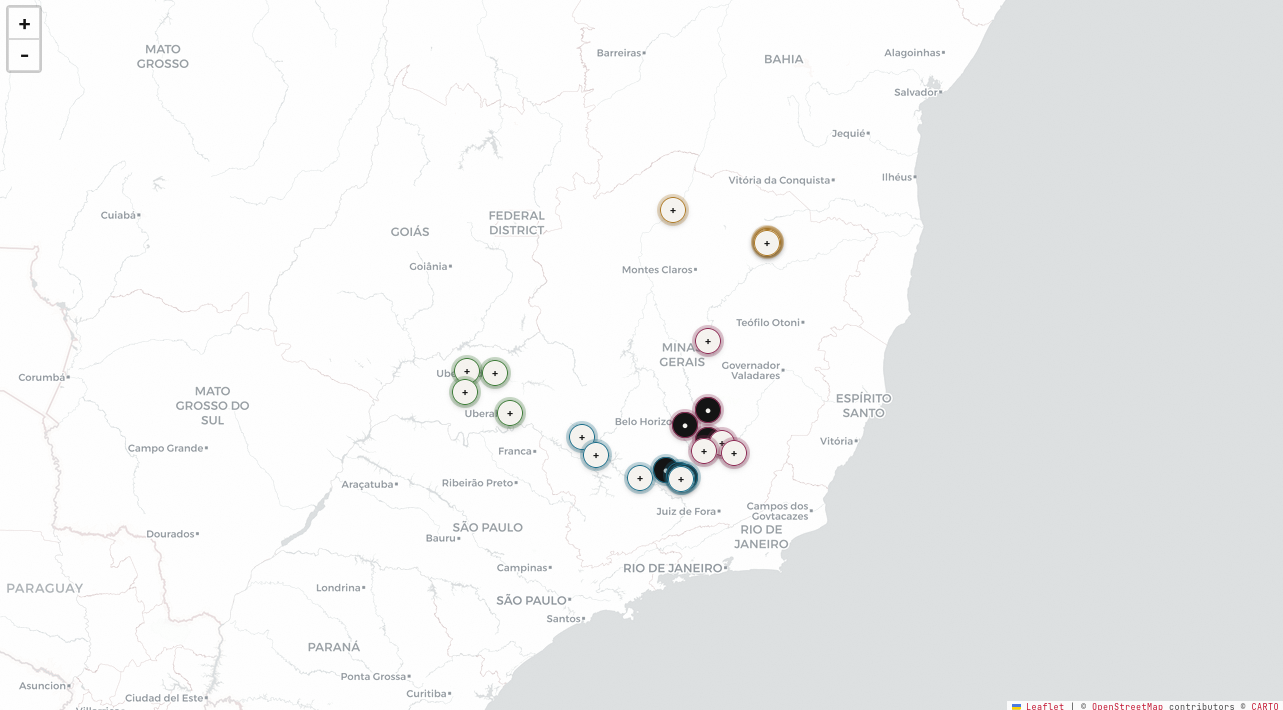
\includegraphics[width=0.485\textwidth, trim={180 40 300 30}, clip]{figuras/communities.png}\hfill
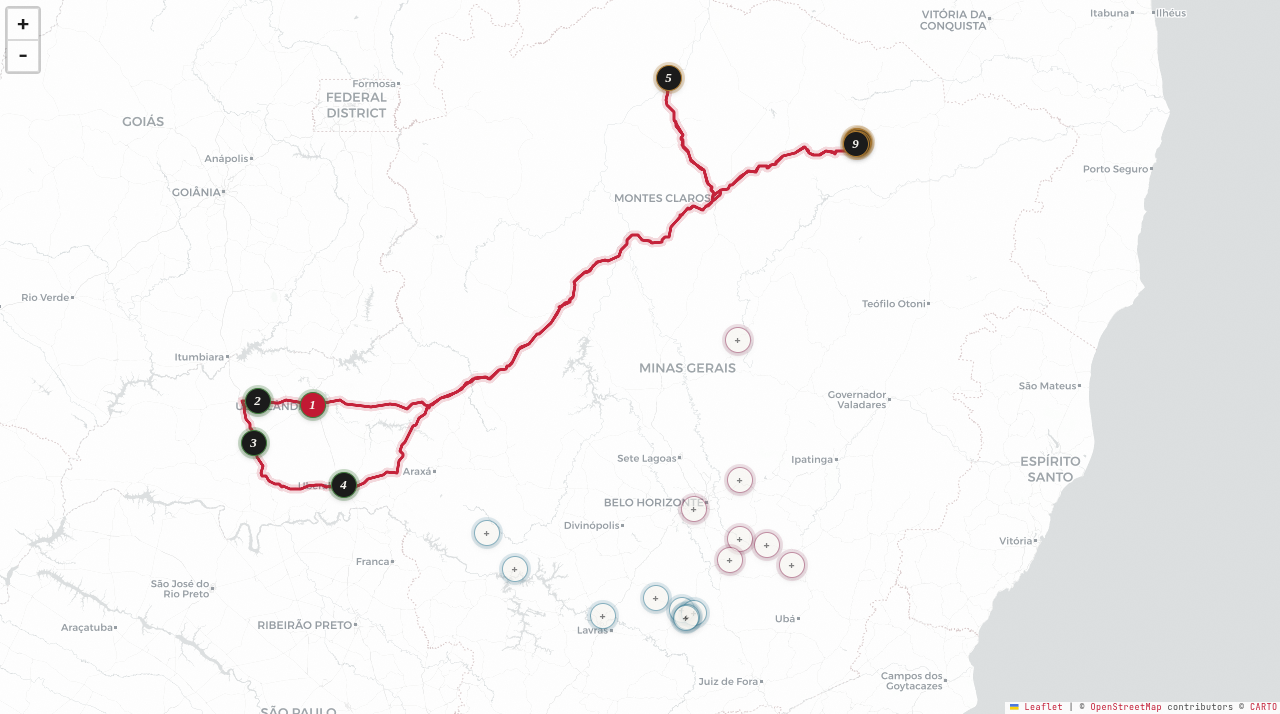
\includegraphics[width=0.485\textwidth, trim={180 40 300 30}, clip]{figuras/route.png}
\caption{À esquerda, os circuitos de visita detectados pelo HP-MOCD no mapa interativo: cada cor de anel corresponde a uma comunidade do grafo de proximidade. À direita, um exemplo de rota gerada pela aplicação, com a ordem de visita numerada e o traçado sobre as estradas reais obtido do OSRM.}
\label{fig:circuitos}
\end{figure*}

O resultado é exposto pelo endpoint \texttt{GET /communities}, que retorna o identificador de comunidade de cada alambique e os grupos formados. No mapa interativo, o usuário pode ativar a visualização dos circuitos: alambiques de uma mesma comunidade recebem um anel de mesma cor, revelando as microrregiões produtoras e apoiando a escolha das paradas antes do cálculo da rota. A Fig.~\ref{fig:circuitos} apresenta os circuitos detectados sobre o conjunto de dados da aplicação, nos quais é possível reconhecer agrupamentos coerentes com regiões produtoras como o Norte de Minas, o Triângulo Mineiro, o Campo das Vertentes e o entorno metropolitano de Belo Horizonte.

\section{Desenvolvimento e Ferramentas}

\subsection{Implementação do Backend}

O backend foi implementado com Node.js, Express e TypeScript. Os endpoints foram organizados por domínio, abrangendo autenticação, alambiques, avaliações, planejamento de rotas, estatísticas do grafo e detecção de comunidades. As requisições são processadas pelos controladores e encaminhadas aos serviços responsáveis pelas regras de negócio.

A autenticação utiliza tokens JWT, enquanto as senhas são protegidas por meio de hash. O sistema também possui middlewares para tratamento centralizado de erros, limitação de requisições e inclusão de cabeçalhos de segurança.

A persistência utiliza o driver oficial do Neo4j e consultas escritas em Cypher. Um script de carga inicial cria as restrições de unicidade e insere no banco as cidades, os alambiques, os usuários, as avaliações e os relacionamentos utilizados na demonstração da aplicação. O conjunto de dados reúne alambiques reais de Minas Gerais distribuídos em cerca de vinte municípios.

\subsection{Interface da API e Consultas Cypher}

A Tabela~\ref{tab:endpoints} resume os endpoints expostos pelo backend. As operações de escrita exigem autenticação por token JWT, enquanto as consultas públicas podem ser acessadas diretamente pela interface.

\begin{table}[t]
\centering
\caption{Endpoints da API do Cachaceiro Viajante. A coluna JWT indica as operações que exigem autenticação.}
\label{tab:endpoints}
{\small
\begin{tabular}{@{}lllc@{}}\toprule
Método & Caminho & Função & JWT\\\colrule
POST & \texttt{/auth/register} & criar conta & --\\
POST & \texttt{/auth/login} & autenticar & --\\
GET & \texttt{/auth/me} & perfil autenticado & sim\\
GET & \texttt{/distilleries} & catálogo paginado & --\\
POST & \texttt{/distilleries} & indicar alambique & sim\\
GET & \texttt{/reviews} & últimas avaliações & --\\
POST & \texttt{/reviews} & registrar avaliação & sim\\
POST & \texttt{/routes/solve} & ordem de visita & --\\
GET & \texttt{/communities} & circuitos HP-MOCD & --\\
GET & \texttt{/stats} & contagens do grafo & --\\\botrule
\end{tabular}}
\end{table}

Como o foco central do trabalho é a modelagem do banco de dados, três consultas ilustram como o modelo em grafos é criado, restringido e percorrido na prática. A Query~\ref{lst:constraint} mostra uma das restrições de unicidade definidas na carga inicial, que garante a integridade dos identificadores diretamente no SGBD.

\begin{lstlisting}[caption={Restrição de unicidade definida sobre os nós \texttt{Distillery}.}, label={lst:constraint}]
CREATE CONSTRAINT distillery_id
IF NOT EXISTS
FOR (d:Distillery)
REQUIRE d.id IS UNIQUE
\end{lstlisting}

A Query~\ref{lst:dist} produz a matriz de distâncias utilizada pelo planejador de rotas e pelo grafo de proximidade da detecção de comunidades, calculando a distância geodésica entre todos os pares de alambiques selecionados por meio do tipo espacial \texttt{point}.

\begin{lstlisting}[caption={Cálculo das distâncias par a par com a função espacial \texttt{point.distance}.}, label={lst:dist}]
MATCH (a:Distillery), (b:Distillery)
WHERE a.id IN $ids AND b.id IN $ids
  AND a.id < b.id
RETURN a.id AS aId, b.id AS bId,
  point.distance(a.location,
                 b.location) AS meters
\end{lstlisting}

Por fim, a Query~\ref{lst:suggest} registra a indicação de um novo alambique por um usuário, criando em uma única operação o nó do estabelecimento, o relacionamento de autoria da indicação e o vínculo com a cidade, reutilizada quando já existente por meio de \texttt{MERGE}.

\noindent\begin{minipage}{\columnwidth}
\begin{lstlisting}[caption={Indicação de um alambique: criação do nó e dos relacionamentos \texttt{SUGGESTED} e \texttt{LOCATED\_IN}.}, label={lst:suggest}]
MATCH (u:User {id: $userId})
MERGE (c:City {name: $city})
CREATE (d:Distillery {id: $id,
  name: $name, status: 'IN_VALIDATION',
  location: point({latitude: $lat,
                   longitude: $lon})})
CREATE (u)-[:SUGGESTED
            {at: datetime()}]->(d)
CREATE (d)-[:LOCATED_IN]->(c)
\end{lstlisting}
\end{minipage}

Consultas desse tipo evidenciam a aderência do modelo em grafos ao domínio: os relacionamentos são criados e percorridos diretamente, sem tabelas intermediárias, as restrições de integridade são declaradas no próprio banco e as coordenadas ficam armazenadas como propriedades espaciais consultáveis pelo SGBD.

\subsection{Implementação do Serviço de Detecção de Comunidades}
\label{sec:impl-comunidades}

A detecção de comunidades foi implementada como um microsserviço em Python, mantido em um contêiner próprio. O serviço utiliza Flask para expor um único endpoint HTTP, que recebe a lista de arestas do grafo de proximidade, monta o grafo com a biblioteca NetworkX e executa o HP-MOCD por meio da biblioteca \texttt{pymocd} \cite{Santos2025}. A resposta associa cada alambique ao identificador de sua comunidade.

No backend Node.js, o serviço de circuitos consulta os alambiques e as distâncias no Neo4j, monta as arestas dos três vizinhos mais próximos de cada estabelecimento e delega o cálculo ao microsserviço. Como o conjunto de estabelecimentos muda com pouca frequência, o resultado é mantido em cache por cinco minutos, evitando reexecuções do algoritmo a cada requisição. Caso o microsserviço esteja indisponível, o backend responde com um erro explícito e o restante da aplicação permanece funcional.

\subsection{Implementação do Frontend}

A implementação da interface utiliza componentes funcionais e serviços responsáveis pela comunicação com o backend por meio de requisições HTTP. Após a autenticação, o token recebido é incluído nas requisições das funcionalidades protegidas, como o registro de avaliações e a indicação de novos alambiques.

No planejamento de rotas, o frontend envia ao backend os identificadores dos estabelecimentos selecionados e o ponto de partida. Após receber a sequência de visita calculada, a aplicação solicita ao OSRM a geometria do trajeto e apresenta o resultado no mapa.

Na tela de planejamento, um controle adicional permite ativar a visualização dos circuitos de visita. Ao ser acionado, o frontend consulta o endpoint de comunidades e passa a colorir os marcadores do mapa conforme o grupo detectado, indicando também a quantidade de circuitos encontrados. A visualização pode ser ativada e desativada sem interferir na seleção de paradas ou na rota calculada.

Caso o serviço de geometria viária não esteja disponível, a interface pode apresentar uma representação simplificada entre os pontos, mantendo a sequência calculada pelo sistema.

\subsection{Ambiente e Ferramentas de Apoio}

O ambiente de execução foi organizado utilizando Docker ou Podman Compose. A infraestrutura é composta por containers destinados ao Neo4j, ao backend, ao carregamento inicial dos dados, ao microsserviço de detecção de comunidades e ao frontend. Essa organização facilita a configuração e a reprodução do ambiente em diferentes máquinas.

Um arquivo Makefile reúne comandos para instalação das dependências, inicialização dos serviços, carregamento do conjunto inicial de dados, execução de testes e visualização dos registros dos containers. O código-fonte e a documentação do projeto são armazenados e versionados em um repositório Git.

\subsection{Disponibilidade do Código-Fonte e da Demonstração}

O código-fonte completo da aplicação, incluindo as instruções necessárias para sua execução, está disponível em um repositório público no GitHub, no endereço \url{https://github.com/glermFF/TP_Bancos_de_Dados_II} \cite{cachaceirogithub}. Também foi disponibilizado um vídeo demonstrativo com a apresentação das principais funcionalidades do sistema \cite{cachaceirovideo}.

\section{Considerações Finais}

Este trabalho apresentou o desenvolvimento do Cachaceiro Viajante, uma aplicação voltada à consulta de alambiques e ao planejamento de roteiros de visita em Minas Gerais. A solução integra uma interface de usuário, um backend responsável pelas regras de negócio, um microsserviço de detecção de comunidades e um banco de dados orientado a grafos. A utilização do Neo4j permitiu representar diretamente as relações entre usuários, avaliações, alambiques e cidades, além de armazenar as coordenadas empregadas no cálculo da ordem aproximada de visita. A geometria viária é obtida posteriormente pelo OSRM e apresentada ao usuário em um mapa interativo.

A incorporação do HP-MOCD \cite{Santos2025} mostrou que o mesmo grafo utilizado para o planejamento de rotas pode alimentar técnicas de análise de redes: a partição em comunidades do grafo de proximidade dos alambiques produz circuitos de visita coerentes com a distribuição geográfica dos estabelecimentos, apresentados ao usuário diretamente no mapa.

Como possibilidades de evolução, destacam-se a implementação de um processo administrativo para validação dos alambiques indicados, a personalização dos roteiros conforme as preferências dos usuários, a utilização dos relacionamentos entre cidades diretamente no cálculo dos percursos e a realização de testes com conjuntos maiores de dados. Também poderão ser avaliadas outras estratégias de ordenação de visitas e outras formas de construção do grafo de proximidade utilizado na detecção de comunidades, como a ponderação das arestas pela malha viária real, permitindo comparar a qualidade das rotas e dos circuitos produzidos.

\bibliography{bib}
\bibliographystyle{jaes}

\end{document}
